\chapter{Leviticus 11}

\begin{figure}
  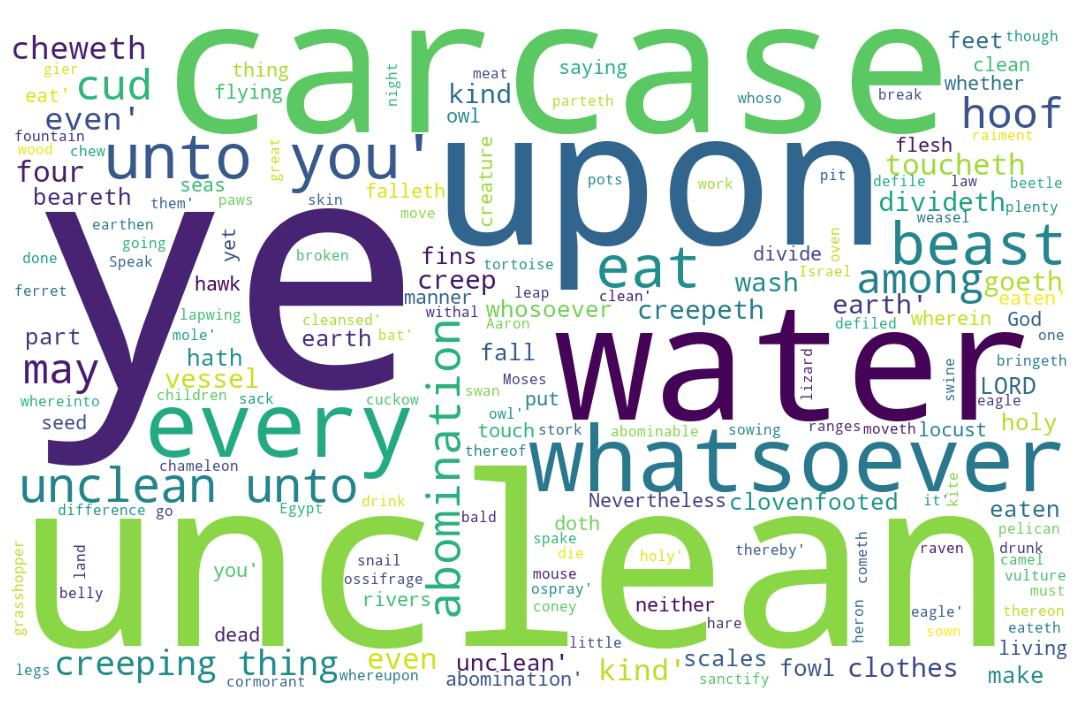
\includegraphics[width=\linewidth]{03OT-Leviticus/Leviticus11-WordCloud.jpg}
  \caption{Leviticus 11 Word Cloud}
  \label{fig:Leviticus 11 word Cloud}
\end{figure}

\marginpar{\scriptsize \centering \fcolorbox{black}{lime}{\textbf{DIFFERENCES \& DIVISION}}\\ (Leviticus 11:1--47) 
\begin{compactenum}[I.][8]
    \item \textbf{Unclean} \index[scripture]{Leviticus!Lev 11:04} (Lev 11:4) (word used 32 times in chapter)
    \item \textbf{Untouchable} \index[scripture]{Leviticus!Lev 11:08}\index[scripture]{Leviticus!Lev 11:24}\index[scripture]{Leviticus!Lev 11:26}\index[scripture]{Leviticus!Lev 11:27}\index[scripture]{Leviticus!Lev 11:31}\index[scripture]{Leviticus!Lev 11:36}\index[scripture]{Leviticus!Lev 11:39} (Lev 11:8, 24, 26, 27, 31, 36, 39)
    \item \textbf{Understanding} \index[scripture]{Leviticus!Lev 11:47} (Lev 11:47) (we must care about this!)
    \begin{compactenum}[A.][7]
    	\item The differences
    	\item The direction
    	\item The determination
    	\item The decisions
    	\item The discernment
    \end{compactenum}
    \item \textbf{Undefiled} (stay undefiled)
    \begin{compactenum}[A.][7]
    	\item In principle
    	\item In practice
    	\item In priority
    \end{compactenum}
    \item \textbf{Unprofitable} (do what makes a difference)
    \item \textbf{Unedifying} 
\end{compactenum} }

%%%%%%%%%%%%%%%%%%%%%%%%%%%%%%
%%%%%%%%%%%%%%%%%%%%%%%%%%%%%%
\footnote{\textcolor[cmyk]{0.99998,1,0,0}{\hyperlink{TOC}{Return to end of Table of Contents.}}}\footnote{\href{https://audiobible.com/bible/leviticus_11.html}{\textcolor[cmyk]{0.99998,1,0,0}{Leviticus 11 Audio}}}\textcolor[cmyk]{0.99998,1,0,0}{And the LORD spake unto Moses and to Aaron, saying unto them,}
[2] \textcolor[cmyk]{0.99998,1,0,0}{Speak unto the children of Israel, saying, These \emph{are} the beasts which ye shall eat among all the beasts that \emph{are} on the earth.}
[3] \textcolor[cmyk]{0.99998,1,0,0}{Whatsoever parteth the hoof, and is clovenfooted, \emph{and} cheweth the cud, among the beasts, that shall ye eat.}
[4] \textcolor[cmyk]{0.99998,1,0,0}{Nevertheless these shall ye not eat of them that chew the cud, or of them that divide the hoof: \emph{as} the camel, because he cheweth the cud, but divideth not the hoof; he \emph{is} \fcolorbox{black}{lime}{unclean} unto you.}
[5] \textcolor[cmyk]{0.99998,1,0,0}{And the coney, because he cheweth the cud, but divideth not the hoof; he \emph{is} unclean unto you.}
[6] \textcolor[cmyk]{0.99998,1,0,0}{And the hare, because he cheweth the cud, but divideth not the hoof; he \emph{is} unclean unto you.}
[7] \textcolor[cmyk]{0.99998,1,0,0}{And the swine, though he divide the hoof, and be clovenfooted, yet he cheweth not the cud; he \emph{is} unclean to you.}
[8] \textcolor[cmyk]{0.99998,1,0,0}{Of their flesh shall ye not eat, and their carcase shall ye \fcolorbox{black}{lime}{not touch}; they \emph{are} unclean to you.}\\
\\
\P \textcolor[cmyk]{0.99998,1,0,0}{These shall ye eat of all that \emph{are} in the waters: whatsoever hath fins and scales in the waters, in the seas, and in the rivers, them shall ye eat.}
[10] \textcolor[cmyk]{0.99998,1,0,0}{And all that have not fins and scales in the seas, and in the rivers, of all that move in the waters, and of any living thing which \emph{is} in the waters, they \emph{shall} \emph{be} an abomination unto you:}
[11] \textcolor[cmyk]{0.99998,1,0,0}{They shall be even an abomination unto you; ye shall not eat of their flesh, but ye shall have their carcases in abomination.}
[12] \textcolor[cmyk]{0.99998,1,0,0}{Whatsoever hath no fins nor scales in the waters, that \emph{shall} \emph{be} an abomination unto you.}\\
\\
\P \textcolor[cmyk]{0.99998,1,0,0}{And these \emph{are} \emph{they} \emph{which} ye shall have in abomination among the fowls; they shall not be eaten, they \emph{are} an abomination: the eagle, and the ossifrage, and the ospray,}
[14] \textcolor[cmyk]{0.99998,1,0,0}{And the vulture, and the kite after his kind;}
[15] \textcolor[cmyk]{0.99998,1,0,0}{Every raven after his kind;}
[16] \textcolor[cmyk]{0.99998,1,0,0}{And the owl, and the night hawk, and the cuckow, and the hawk after his kind,}
[17] \textcolor[cmyk]{0.99998,1,0,0}{And the little owl, and the cormorant, and the great owl,}
[18] \textcolor[cmyk]{0.99998,1,0,0}{And the swan, and the pelican, and the gier eagle,}
[19] \textcolor[cmyk]{0.99998,1,0,0}{And the stork, the heron after her kind, and the lapwing, and the bat.}
[20] \textcolor[cmyk]{0.99998,1,0,0}{All fowls that creep, going upon \emph{all} four, \emph{shall} \emph{be} an abomination unto you.}
[21] \textcolor[cmyk]{0.99998,1,0,0}{Yet these may ye eat of every flying creeping thing that goeth upon \emph{all} four, which have legs above their feet, to leap withal upon the earth;}
[22] \textcolor[cmyk]{0.99998,1,0,0}{\emph{Even} these of them ye may eat; the locust after his kind, and the bald locust after his kind, and the beetle after his kind, and the grasshopper after his kind.}
[23] \textcolor[cmyk]{0.99998,1,0,0}{But all \emph{other} flying creeping things, which have four feet, \emph{shall} \emph{be} an abomination unto you.}
[24] \textcolor[cmyk]{0.99998,1,0,0}{And for these ye shall be unclean: whosoever toucheth the carcase of them shall be unclean until the even.}
[25] \textcolor[cmyk]{0.99998,1,0,0}{And whosoever beareth \emph{ought} of the carcase of them shall wash his clothes, and be unclean until the even.}
[26] \textcolor[cmyk]{0.99998,1,0,0}{\emph{The} \emph{carcases} of every beast which divideth the hoof, and \emph{is} not clovenfooted, nor cheweth the cud, \emph{are} unclean unto you: every one that toucheth them shall be unclean.}
[27] \textcolor[cmyk]{0.99998,1,0,0}{And whatsoever goeth upon his paws, among all manner of beasts that go on \emph{all} four, those \emph{are} unclean unto you: whoso toucheth their carcase shall be unclean until the even.}
[28] \textcolor[cmyk]{0.99998,1,0,0}{And he that beareth the carcase of them shall wash his clothes, and be unclean until the even: they \emph{are} unclean unto you.}\\
\\
\P \textcolor[cmyk]{0.99998,1,0,0}{These also \emph{shall} \emph{be} unclean unto you among the creeping things that creep upon the earth; the weasel, and the mouse, and the tortoise after his kind,}
[30] \textcolor[cmyk]{0.99998,1,0,0}{And the ferret, and the chameleon, and the lizard, and the snail, and the mole.}
[31] \textcolor[cmyk]{0.99998,1,0,0}{These \emph{are} unclean to you among all that creep: whosoever doth touch them, when they be dead, shall be unclean until the even.}
[32] \textcolor[cmyk]{0.99998,1,0,0}{And upon whatsoever \emph{any} of them, when they are dead, doth fall, it shall be unclean; whether \emph{it} \emph{be} any vessel of wood, or raiment, or skin, or sack, whatsoever vessel \emph{it} \emph{be}, wherein \emph{any} work is done, it must be put into water, and it shall be unclean until the even; so it shall be cleansed.}
[33] \textcolor[cmyk]{0.99998,1,0,0}{And every earthen vessel, whereinto \emph{any} of them falleth, whatsoever \emph{is} in it shall be unclean; and ye shall break it.}
[34] \textcolor[cmyk]{0.99998,1,0,0}{Of all meat which may be eaten, \emph{that} on which \emph{such} water cometh shall be unclean: and all drink that may be drunk in every \emph{such} vessel shall be unclean.}
[35] \textcolor[cmyk]{0.99998,1,0,0}{And every \emph{thing} whereupon \emph{any} \emph{part} of their carcase falleth shall be unclean; \emph{whether} \emph{it} \emph{be} oven, or ranges for pots, they shall be broken down: \emph{for} they \emph{are} unclean, and shall be unclean unto you.}
[36] \textcolor[cmyk]{0.99998,1,0,0}{Nevertheless a fountain or pit, \emph{wherein} \emph{there} \emph{is} plenty of water, shall be clean: but that which toucheth their carcase shall be unclean.}
[37] \textcolor[cmyk]{0.99998,1,0,0}{And if \emph{any} \emph{part} of their carcase fall upon any sowing seed which is to be sown, it \emph{shall} \emph{be} clean.}
[38] \textcolor[cmyk]{0.99998,1,0,0}{But if \emph{any} water be put upon the seed, and \emph{any} \emph{part} of their carcase fall thereon, it \emph{shall} \emph{be} unclean unto you.}
[39] \textcolor[cmyk]{0.99998,1,0,0}{And if any beast, of which ye may eat, die; he that toucheth the carcase thereof shall be unclean until the even.}
[40] \textcolor[cmyk]{0.99998,1,0,0}{And he that eateth of the carcase of it shall wash his clothes, and be unclean until the even: he also that beareth the carcase of it shall wash his clothes, and be unclean until the even.}
[41] \textcolor[cmyk]{0.99998,1,0,0}{And every creeping thing that creepeth upon the earth \emph{shall} \emph{be} an abomination; it shall not be eaten.}
[42] \textcolor[cmyk]{0.99998,1,0,0}{Whatsoever goeth upon the belly, and whatsoever goeth upon \emph{all} four, or whatsoever hath more feet among all creeping things that creep upon the earth, them ye shall not eat; for they \emph{are} an abomination.}
[43] \textcolor[cmyk]{0.99998,1,0,0}{Ye shall not make yourselves abominable with any creeping thing that creepeth, neither shall ye make yourselves unclean with them, that ye should be defiled thereby.}
[44] \textcolor[cmyk]{0.99998,1,0,0}{For I \emph{am} the LORD your God: ye shall therefore sanctify yourselves, and ye shall be holy; for I \emph{am} holy: neither shall ye defile yourselves with any manner of creeping thing that creepeth upon the earth.}
[45] \textcolor[cmyk]{0.99998,1,0,0}{For I \emph{am} the LORD that bringeth you up out of the land of Egypt, to be your God: ye shall therefore be holy, for I \emph{am} holy.}
[46] \textcolor[cmyk]{0.99998,1,0,0}{This \emph{is} the law of the beasts, and of the fowl, and of every living creature that moveth in the waters, and of every creature that creepeth upon the earth:}
[47] \textcolor[cmyk]{0.99998,1,0,0}{To make a \fcolorbox{black}{lime}{difference} between the unclean and the clean, and between the beast that may be eaten and the beast that may not be eaten.}